\chapter{Methods}

In the present chapter, the dataset provided for the analysis is first explained. Then, procedures for labelling each MER are detailed followed by the pre-processing approaches for MER to clean the signals. Methodology for extraction of features, both directly from signal and from neuro-physiological information (spikes), are described in sections~\ref{sec:spkFeat} and~\ref{sec:tfnFeat}.  and constracted tools related is explained in the following sections.  

\section{Microelectrode Recordings}

	Our signals dataset was collected from 5 PD patients undergoing bilateral STN-DBS using three electrodes in each hemisphere -central, lateral and anterior channels. Recordings started 10 mm above the estimated target and ended approximately 3.5 mm after, thus signals were acquired at around 23 different depths in each channel, as shown in figure \ref{fig:datasret}. Acquisitions were sampled at 24 kHz per channel, filtered (band-pass filtering, 0.5-5 kHz) and amplified, previously to their storage. Duration of recorded signal varies between patients, since two of the patient's registers lasted for 30 seconds of duration at each depth while the rest of the recordings lasted for 10 seconds.
	
\begin{figure}[!htb]
     \centering    
         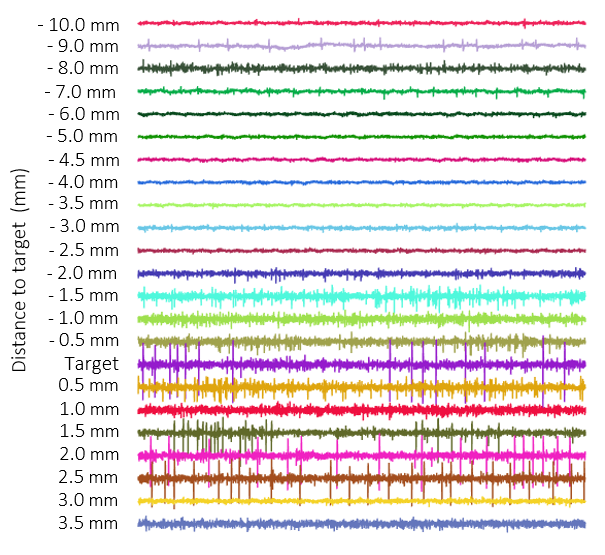
\includegraphics[width=0.7\textwidth]{depthsRN.png} 

       \caption{Segments of MERs (500 ms duration) at each depth along the trajectory with central electrode, starting recordings from 10 mm above target to 3.5 mm under.}
     \label{fig:datasret}
\end{figure} 

\textit{Table with patients data is important and where?. }
\subsection{Imagiology}

\textit{Is it necessary to describe provided\textbf{ images details and target coordinates in Z} here or is it better only in anatomically-based classification section???}


\section{Localisation of electrode position for MER labelling}

Labelling each MER of our dataset regarding its position is important in order to effectively identify features for distinguish STN from non-STN MER and to  to construct the automatic classifier. Therefore, different approaches are explored for labelling MER regarding its location within the target, both further explained in the following sections. First approach is based on unbiased visually inspection and classification of MER segments within STN by an expert. Second labelling is based on lead trajectory localization reconstruction using individual patient imagiology, fused with an STN functional subdivision atlas. Gold-standard classification could be obtained through this approach and it allows us to compare physiological neurons properties in motor/non-motor STN.

%\textit{Labelling each signal regarding its position in relation to the STN is essential. Thefore, all recordings are identified and labelled through two different approaches: visual inspection by an expert and based on patient's fused imagiology. Both procedures are further explained following.  Both approaches are further explained}



%Labels of STN subterritories, and gold standard labelling is based on 

%Neuroimaging
%Regarding the assesment of the 
%Patiet's magnetic resonance imaging (MRI) is studied in order to evaluating the patient's 
%defined labels and based on trajectory localization reconstruction
% acquired along the intraoperative trajectory are 

%Furthermore, in this study  patient's imagiology is also used to identify each localization of the microelectrode recordings along their trajectory. This data is important in order to correctly classify ----------
%Therefore, gold-standard classification of could be obtained through this approach and it allow us to based on patient's imagiology. 
%\subsection*{Localisation of electrode tip within the area of interest}
%Datos sobre la localizacion del electrodo en cada una de las señales son esenciales para la construccion de un classificador automatico. Por lo tanto 


\subsection{Expert-based classification}

Labels regarding each signal's position within the STN were identified  through visual inspection by an expert. In order to facilitate visualization and labelling of all signals and to preserve the classification unbiased to previous knowledge about MER depths, a customized script in Matlab was programmed. 

This script first shuffles all signals in the dataset and it plots in random order one signal at a time. The whole signal and two enlarged segments (1 second and 500 milliseconds duration, randomly chosen from the raw signal) are shown to classify, as shown in figure~\ref{fig:classifSgignals} for each signal in the dataset. Then, the expert is asked to identify the current signal as \textit{STN (1)}, \textit{not-STN (2)} or \textit{try again (3)}. If any signal is classified as \textit{try again} for the first time, it is shown again until the third attempt, when it is classified as \textit{unclear (3)}. 

Additionally for each signal classified as STN, the expert is asked to set its value of certainty of its localization from 1 (very unclear) to 5 (high certainty), which gives an idea of the confidence of each classification for further analysis.
 
\begin{figure}[!htb]
     \centering    
         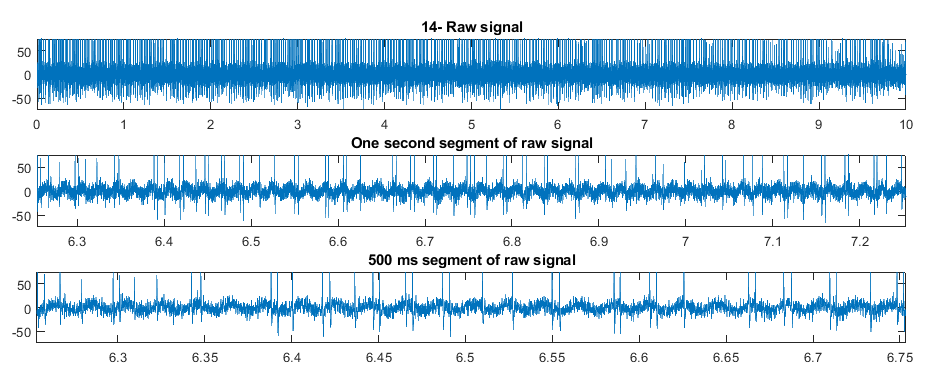
\includegraphics[width=0.7\textwidth]{selectionSignals.png} 

       \caption{Segments of MERs (500 ms duration) at each depth along the trajectory, starting recordings from 10 mm above target to 3.5 mm under.}
     \label{fig:classifSgignals}
\end{figure} 

\textit{Numbers of classification results (table) should be shown in results, right? } 
 
However, labelling subterritories of STN based on visual inspection is not a viable option since differences are not clearly discernible. Accordingly, this subdivision is manually defined by splitting the consecutive recordings identified as STN along each trajectory into three equal parts: dorsal, medial and ventral part of STN. Then, signals classified as borders of STN are discarded also with the medial ones, resulting in labels for both dorsal and ventral regions, probably motor and non-motor STN respectively. 


\subsection{Anatomically-based classification}

Reconstruction of trajectory localization for each lead presents a gold-standard approach, since it is based on both pre-operative and post-operative patient's imagiology fused to an atlas of STN functional subterritories. In order to localise the electrode tip and trajectory and also for patient's image processing, LeadDBS, a Matlab toolbox [\url{http://www.lead-dbs.org}; \cite{Horn2015}] were applied in this approach. Along with this software, Slicer3D [\url{https://www.slicer.org/}] is also used to import all images into Nifty, which were provided in DICOM.

Afterwards and through Lead DBS, MRI images are coregistered using SPM12 method [\url{http://www.fil.ion. ucl.ac.uk/spm/software/spm12/}], whereas post-operative contrast-enhanced computed tomography (CT) image was coregistered to preoperative MRI images with Advanced Normalization Tools [ANTs; \url{http://stnava.github.io/ANTs/}]. All volumes are later normalized to standard stereotactic space (MNI; ICBM152 2009b non-linear asymmetric) using Dartel implemented in SPM.

\begin{figure}[!htb]
     \centering    
     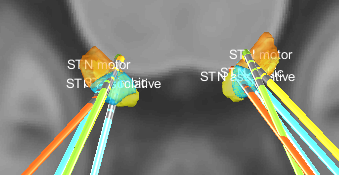
\includegraphics[width=0.7\textwidth]{stnReconstruct.png}
       \caption{Axial view of STN subdivisions with reconstructed electrodes based on each patient’s images through Lead DBS }
     \label{fig:spkSorting}
\end{figure}

In order to obtain electrode's location and trajectory, reconstruction is manually supervised assessed with pre-reconstruction through PaCER method and Acolla's STN subterritories atlas \cite{Accolla2014, Husch2018}. Once definitive coordinates of electrode are located, MER localizer tool in LeadDBS is used to determinate locations along the trajectory in all channels.

%Image specifications (acquisition) here? Lead DBS and Slicer methodology
%More accurate localization of recordings at each depth is estimated through reconstruction of the trajectory for each implanted lead with both fused pre-operative and post-operative patient's images and STN functional subdivisions \cite{Accolla2014} atlas.
%Reconstruction of trajectory will be performed through LeadDBS using STN subdivisions atlas reconstructed on patient’s 
%pre-operative MRI and pos-operative CT previously co-registered.
%Furthermore,  haciendo uso de (con recurso a) las fused images del pre and post operative images paciente se realizó otra classificacion, siendo asi considerada como gold standard. A través de estas señales y con la identificacion del posicionamento y el canal utilizado definitivo, se pueden obtener las diferentes posiciones de cada uno de los electrodos y canales along the route.
%Para esta classificacion se utilizo la toolbox de matlab Lead DBS software blabla, especializada ya en la reconstruccion de electrodos?
% Postoperative electrode reconstructions are performed using Lead-DBS toolbox [\url{http://www.lead-dbs.org}; %\cite{Horn2015}], implemented in Matlab. % [http://www.lead-dbs.org; Horn and K€uhn, 2015; RRID:SCR_002915] in Matlab.Along with this software, Slicer3D [\url{https://www.slicer.org/}] is also used to import all images into Nifty, which were provided in DICOM.
% of the  Una vez obtenida la localizacion definitiva del electrodo, la herramienta MER recoerdings? es utilizada para determinar la localizacion de los otros dos canales con trayectoria paralela utilizados (anterior y lateral) y asi obtenemos el posicionamiento para cada uno de nuestras profundidades y 
%Exporting DICOM images into Nifty performed com recurso a Slicer 3D. Postoperative electrode localizations were performed using Lead-DBS software % [http://www.lead-dbs.org; Horn and K€uhn, 2015; RRID:SCR_002915] in Matlab.
%First, MRI images were coregistered using SPM method () whereas post-operative CT was coregistered to preoperative MRI images with ANTs.
%Afterwards, volumes were normalized with SPM Shoot???.
%In order to obtain electrode's location and trajectory, reconstruction is manually supervised assessed with pre-reconstruction through PaCER method.

\section{Filtering MER and artefact detection}
\label{sec:filtering}
Some noisy signals are present in MER dataset with different types of artefacts. According to \citeA{Bakstein2017}, noise in MER may affect more than 25\% of the recording length and can arise due to a number of factors such as mechanical movement manifested by high power signal peaks, electromagnetic interference such as the 50 Hz interference from the power grid, low-frequency interferences ($<$50 Hz) and "irritated neurons" with high spiking activity. Consequently, pre-processing these signals is an important step in order to avoid errors in the extracted features and .

Filtering the signal is our first step in this pre-processing part, since it can smooth out high-frequency fluctuations and/or remove periodic trends of a specific frequency from data. Therefore we filter the data using an elliptic band-pass filter between 300 and 5000 Hz. Elliptic filter was chosen after visual inspection of different types of signals and its effects on spike detection, since it keeps waveforms of firing neurons unaltered \cite{QuianQuiroga2009}. Implemented filter of order 4 is set to 0.6 decibels (dB) of peak-to-peak ripple and 60 dB of attenuation and it is performed with zero-phase digital filtering in order to preserve time features. Nevertheless, all parameters can be easily modified in our tool and also code for testing other types of filters is implemented.

\begin{figure}[!htb]
     \centering    
              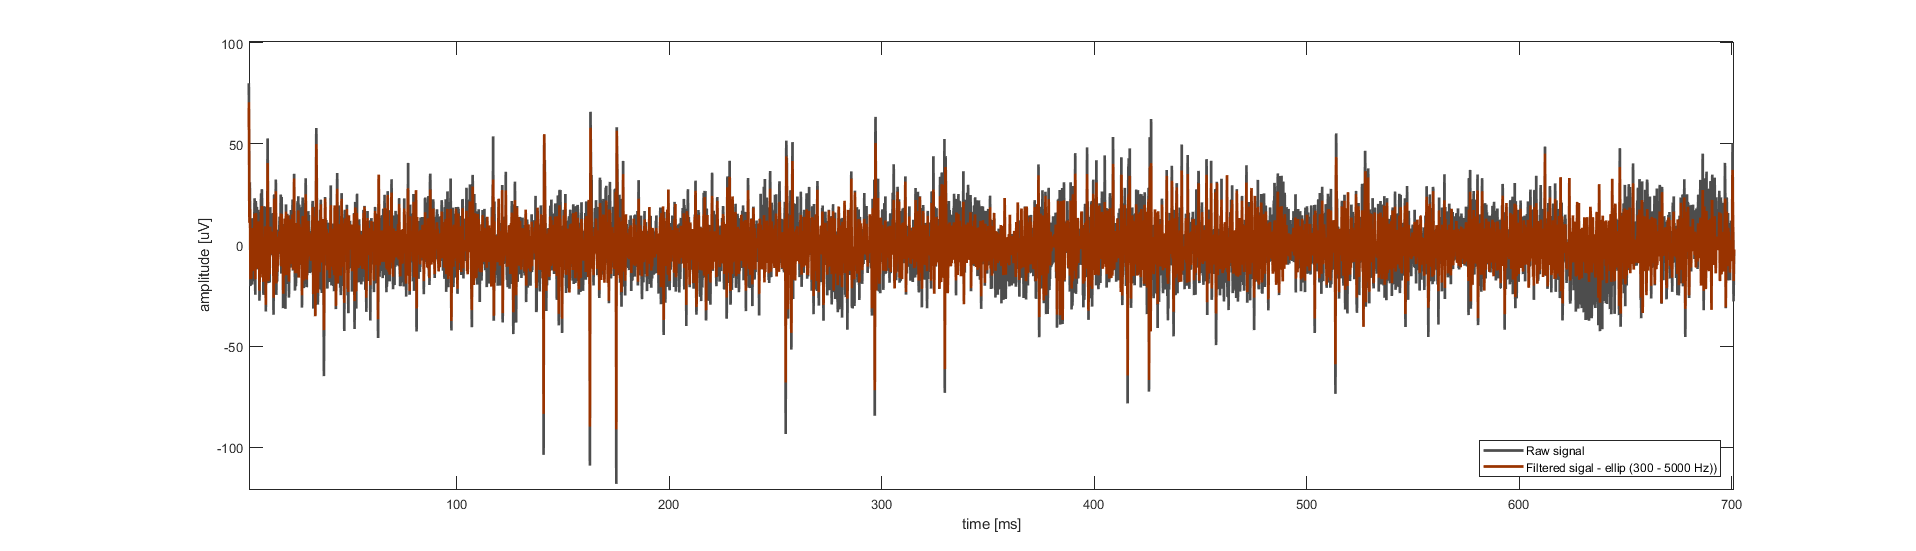
\includegraphics[width=0.7\textwidth]{filtered_700ms.png} 
       \caption{Filtered signal (700 ms) with elliptical filter overlapped to raw MER.}
     \label{fig:artifacts}
\end{figure}

In addition to the filtering, we reviewed previous approaches for MER artifact removal literature and visually inspected their performances on our dataset \cite{OShea2017, Bakstein2017, Grubhoffer2016}. Best observed approach for artifact detection was found with autocorrelation-based method from \citeA{Bakstein2017}. We  adapted their open-source algorithm in order to extract both the longest consecutive segment and a clean signal with the detected artefacts cropped? out, as illustrated in figure~\ref{fig:artifacts}

\begin{figure}[!htb]
     \centering    
       \caption{Reconstructed electrode trajectory with STN subdivision atlas}
     \label{fig:artifacts}
\end{figure}



\section{Extraction of features related with time, frequency and noise}
\label{sec:tfnFeat}

Differences between raw signals along the trajectory to target are discernible through visual inspection as shown before, therefore signal characteristics calculated through computational analysis might reflect these variations. Consequently features related with time, frequency and noise are extracted from filtered MER in order to find features for distinguishing STN from non-STN recordings.

Custom Matlab code was implemented to first load the table dataset with all MER data used, since following analysis and feature extraction is performed one signal at a time and extracted values for each signal are stored in a table along with recording data, all in an unsupervised way after setting input parameters. 

For each MER, the raw signal is first filtered as explained in section~\ref{sec:filtering} and then, if artefact detection and removal is performed, it is inspected and it results in a segment of cleaned signal from interferences. 

Segment of MER to analyse (or whole signal) is divided in smaller segments to extract its characteristics based on statistics of all segment's calculated features. This division in frames should provide a more robust approach for signals with noisy signals or high variability within the same signal vs. extraction of characteristics from the whole signal. Therefore, we split the signal into frames of 2048 samples overlapped 50\% (1024 samples) with Hanning windows, resulting in more than 230 segments for each 10 second signal (sampled at 24 kHz). 

Features related with time are then obtained directly from each frame: \textit{mean absolute value} (MAV), \textit{mean absolute value slope} (MAVS), zero crossings (ZC), \textit{RMS power} (Prms), \textit{waveform of curve length} (WL), \textit{variance} (var), \textit{Teager energy} (TE) and \textit{crest factor} (CrF). In relation to noise, two measures were obtained:an estimation of \textit{standard deviation of noise} (spN) and \textit{signal-to-noise ratio} (SNR). Features related with frequency domain are: \textit{spectral centroid} (spC), \textit{spectral roll off} (sRO), \textit{spectral flux}, \textit{mean frequency} (mFreq), \textit{median frequency} (medFreq) and \textit{12 Mel coefficients}. Features definition and formulas of extracted parameters are presented in appendix X.
% filtered MER divided in smaller segments through a custom Matlab code. Secondly, features based on neuronal activity from firing neurons, shown in MER as spike events as in figure 2, are calculated. Beforehand, spike events are detected from filtered signal and since they may be originated from more than one different neuron, spike sorting is performed identifying one cluster for each neuron, based on their spike waveforms and selected features. Preliminary probability tests with some extracted features show significant differences, as illustrated in figure 3 for STN identification and figure 4 regarding dorsal STN. 

\section{Features related with neuronal activity }
\label{sec:spkFeat}
Microelectrodes register neuronal activity, part of which consists of action potentials (AP), spikes generated from neurons in the nearest region of the electrode tip as already mentioned in section~\ref{sec:electroph}. Therefore, different depths of the brain show different neuronal activity and consequently, related characteristics are studied based on the detected spikes to extract relevant neurophysiological properties for target identification in STN-DBS.

Nevertheless, prior to the spike-related features quantification, action potentials of the different neurons are detected from the MER as spiking events by a process known as spike detection, further explained in section~\ref{sec:spkDetection}. Afterwards, different neurons are separated in different clusters, process detailed in section~\ref{sec:spkSorting} known as spike sorting. Extraction of their features is implemented lastly, once neurons are sorted and detected from each MER.

%\subsubsection{Spike features}
\textit{Algorithms for Spike Detection and Sorting. Should I explain them in detail? And here or in discussion/results when talking about modified parameters?}

\subsection{Spike detection}
\label{sec:spkDetection}
In this process, firing neurons are detected as spike events from the filtered signal. The used algorithm is Spike Detection with Continuous Wavelet Transform \cite{Nenadic2008}
 This algorithm uses the continuous wavelet transform (CWT) combined with information about the typical interval duration of AP to identify these spiking events. Biorthogonal family was used with this algorithm, though it can be used with other types of wavelets, but this family presents bi-phasic phase which is similar to APs, as illustrated in figure~\ref{fig:spkDetection}A,  and when translated and scaled, a bank of approximately matched filters for AP identification along the signal is formed.
 
\begin{figure}[!htb]
     \centering    
               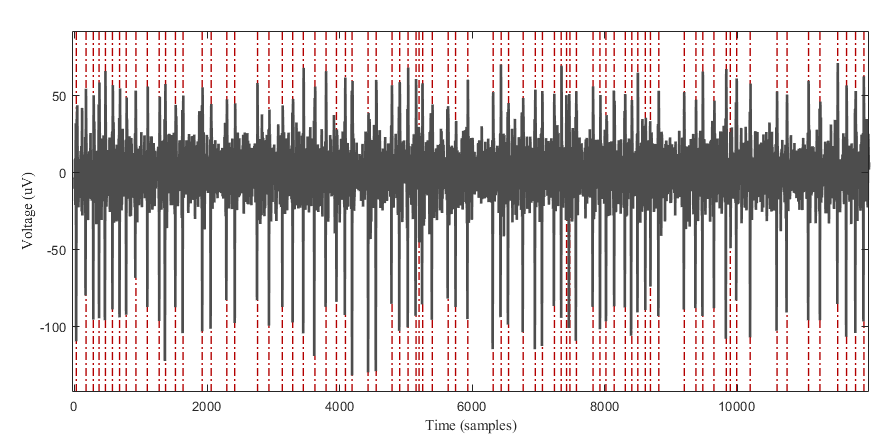
\includegraphics[width=0.9\textwidth]{spkDetection.png} 
       \caption{A)  Typical waveforms of action potentials (top) and biorthogonal wavelet family (bottom). B) Spike train of detected spike events (red) on the clean filtered signal (gray).}
     \label{fig:spkDetection}
\end{figure} 
 \textit{ Missing figure of wavelet vs. typical action potential shape! 
 Explain more deeply about wavelet or this algorithm?}
 
 Nenadic's algorithm was chosen instead of threshold detection, which is more widely used, since it presented better performance with an unsupervised approach on the number of detected spikes versus threshold detection (both fixed and adaptative) in noisy signals. This may be due to the fact that this method is less affected by the highly variability of amplitudes and background noise between all signals and more stable for unsupervised analysis. 
 
  \subsection{Spike sorting}
 \label{sec:spkSorting}
 Detected firing events within the same signal may be originated from more than one different neuron and consequently it is important to correctly identify their origin in order to avoid misclassifications and errors in the spike related features. Thus and as mentioned before, spike sorting consists in grouping the detected spikes into clusters based on the similarity of their waveforms.

Since we aim to develop an unsupervised tool for neurophysiological features extraction based on MER, we research the spike sorting literature in order to find a suitable algorithm to adapt to our analysis tool. Therefore our spike sorting is performed with Linear Discriminant Analysis and Gaussian Mixture Model (LDA-GMM) and outlier detection, through an available algorithm and implemented code in Matlab from \citeA{Keshtakaran2017}. 
This method using subspace learning applies LDA to extract most discriminative features from the spike waveforms and performs clustering with automatic detection of the number of the clusters based on GMM.
(Write more about LDA GMM).
Parameters adjustment (since used parameters were not defined by default...is explained better in results and mentioned here?)

\begin{figure}[!htb]
     \centering   
      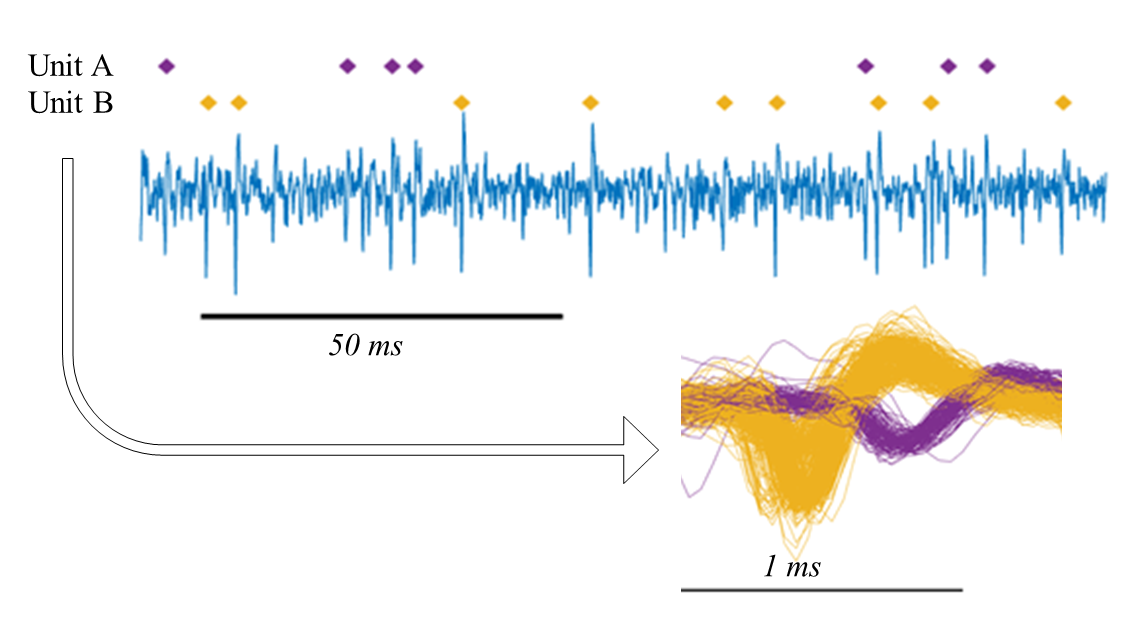
\includegraphics[width=0.75\textwidth]{spkSorting.png} 
       \caption{Detected spikes in filtered MER after spike detection and sorting (top) and their respective overlapped waveforms (bottom).}
     \label{fig:spkSorting}
\end{figure}  

In order to address the quality of each cluster in an objective and standardized way, different related measures are extracted through existing algorithms. Therefore and regarding the isolation quality for each cluster, isolation score is quantified as explained in \cite{Joshua2007}. This score measures the overlap between the noise and the spike clusters. Also with the same algorithm, an estimation of the proportion of false positive and false negative classification errors is obtained.

\subsection{Spike related features extraction}

Based on each neuron's spike train, related features are extracted again through custom Matlab code. Different groups can be distinguish with some of these characteristics according to the measurement unit related with. Specifically, three types of spike features are determined quantifying spike train oscillations, periodicity of spike trains and bursting-related neurons. 

In spite of these groups, \textit{Firing rate} is extracted as a measure of the number of spikes per unit.  \textit{Fano factor} quantifies the variability of the increments of a spike train, and it was calculated according to the literature \cite{Llc2005}. Median values of \textit{Spike maximum amplitude} and \textit{Spike peak-to-peak amplitude} are also stored as measurements of spikes events amplitude. 
 
 A group of features is based on periodicity of the spike trains, specifically related with the \textit{Inter-Spike Interval} (ISI).
%and consequently with the(?) Firing Rate (FR). 
 These features are \textit{Modified burst index} (MBI), \textit{Pause index} (PI), \textit{Pause ratio} (PR), \textit{Bursting index} (BI), \textit{Assimetry index} (AI), \textit{median ISI} (medISI) and \textit{coefficient of variation of ISI} (cvISI).
 
 Spike train oscillations characteristics are also studied through two different approaches. Since neuronal oscillations are typically separated into bands of frequency, these related features are also calculated for each range. Therefore, these bands of neuronal oscillatory activity are: delta (1–4Hz), theta (4–8Hz), alpha (8–12Hz), beta (12–30 Hz), and gamma (30–80Hz). \textit{Modulation indexes} and their significance are calculated through available algorithm and code \citeA{Matzner2015} . On the other hand, features quantifying the oscillation frequency and strength in the given band through the \textit{Oscillation score} and \textit{Oscillation frequency} through the method from \citeA{Muresan2008}.

\begin{figure}[!htb]
     \centering   

       \caption{Spike train and detected bursts through Rank Surprise algorithm}
     \label{fig:bursts}
\end{figure}  

Lastly, characteristics related with bursting neurons are calculated after bursts are previously detected through the Rank Surprise Algorithm, which is based on ISI for detecting bursts \cite{Gourevitch2007}. Extracted features from bursting neurons are: \textit{Burst rate} (BR), \textit{Burst duration} (BD), median \textit{Inter-burst interval} (interBI) and \textit{Intra burst frequency} (intraBI).


%De Vaz ECP: sincronizaçao dos circuitos provocada pela perda de dopamina relacionava-se com o aparecimento de um padrõ oscilarotio na banda beta (11-30 hz) qu era revertido com a alta frequencia na ecp e pela activaçao dopaminergica    ver pag 26 livro 


\section{Classification with Machine Laerning }
Automatic identification of the signals recorded in the Subthalamic Nucleus and specifically its sensorimotor part will be implemented trough machine learning techniques and using the previously extracted features also combined with the information of the electrode's localization for each depth along the trajectory to the area of interest.

%In order to identify these signals recorded from the STN and since multiple approaches are explored in the localisation and feature extraction, also different options and methods will be inspected to find the best classification performance to identify both the STN and furthermore, its motor subdivision. 
Nevertheless, this classification methods require both training and methodological testing and therefore big amount of data is necessary. It is in this matter mostly where your collaboration is essential for a good classification performance with high values of accuracy, sensitivity and sensibility.

Normalization of features?accros series using z-score
